% $Header: /cvsroot/latex-beamer/latex-beamer/solutions/conference-talks/conference-ornate-20min.en.tex,v 1.6 2004/10/07 20:53:08 tantau Exp $

\documentclass[11pt),table]{beamer}
\usepackage{xcolor}
% This file is a solution template for:

% - Talk at a conference/colloquium.
% - Talk length is about 20min.
% - Style is ornate.

% Copyright 2004 by Till Tantau <tantau@users.sourceforge.net>.
%
% In principle, this file can be redistributed and/or modified under
% the terms of the GNU Public License, version 2.
%
% However, this file is supposed to be a template to be modified
% for your own needs. For this reason, if you use this file as a
% template and not specifically distribute it as part of a another
% package/program, I grant the extra permission to freely copy and
% modify this file as you see fit and even to delete this copyright
% notice. 
\usepackage{color}

%\usepackage{wasysym}
%\usepackage{movie15} 
\newcommand{\red}[1]{\textcolor{red}{#1}}
\newcommand{\green}[1]{\textcolor{green}{#1}}
\usepackage{tikz}
\usetikzlibrary{bayesnet}

\definecolor{curie}{rgb}{1,0.4,0}

% pastel colors (latent nodes)
\definecolor{lavender}{rgb}{0.67,0.5,1.0}
\definecolor{cream}{rgb}{0.96,0.8,0.69}
\definecolor{tomato}{rgb}{1.0,0.41,0.41}
\definecolor{lightpink}{rgb}{1.0,0.75,0.796}
\definecolor{SpringGreen}{rgb}{0.5,1.0,0}
\definecolor{anis}{rgb}{0.858,0.858,0.44}
\definecolor{lightBlue}{rgb}{0.59,1.0,1.0}
\definecolor{blue}{rgb}{0.36,0.67,0.93}


% dark colors (observed nodes)
\definecolor{DarkViolet}{rgb}{0.28,0.24,0.545}
\definecolor{DarkBlue}{rgb}{0.06,0.3,0.545}
\definecolor{DarkRed}{rgb}{0.545,0.137,0.137}
\definecolor{DarkBrown}{rgb}{0.36,0.2,0.09}
\definecolor{DarkGreen}{rgb}{0,0.39,0}
\definecolor{DarkPink}{rgb}{0.545,0.04,0.31}


\tikzset{
  treenode/.style = {align=center, inner sep=0pt, text centered,
    font=\sffamily},
  grey_node/.style = {treenode, circle, white, font=\sffamily\bfseries, draw=black,
    fill=grey, text width=1.5em},% noeud gris (observation)
  red_node/.style = {treenode, circle, red, draw=red, 
    text width=1.5em, very thick},% noeud rouge (paramètre)
 white_node/.style = {treenode, circle, black, draw=black, 
    text width=1.5em, very thick},% noeud rouge (paramètre)
  arn_x/.style = {treenode, rectangle, draw=black,
    minimum width=0.5em, minimum height=0.5em}% arbre rouge noir, nil
}

\usetikzlibrary{positioning,shapes,shadows,arrows}

% couleur curie

  \usetheme{Boadilla}
  % or ...

  \setbeamercovered{transparent}
  % or whatever (possibly just delete it)

\setbeamertemplate{navigation symbols}{}

\usepackage[utf8]{inputenc} 	% L'encodage. Ca peut être à remplacer par \usepackage[utf8]{inputenc}
\usepackage[T1]{fontenc}
\def\ques{\noindent{\bf Question : }}
\usepackage[english]{babel}

\usepackage[utf8]{inputenc}
% or whatever

\usepackage{times}
\usepackage[T1]{fontenc}
% Or whatever. Note that the encoding and the font should match. If T1
% does not look nice, try deleting the line with the fontenc.
\usepackage{graphics}

\title % (optional, use only with long paper titles)
{Estimation par maximum de la composite likelihood des parametres du modèle Poisson log-normal}

\subtitle{Mémoire de M2 réalisé sous la supervision de Stéphane Robin}

\author[Elsa TEULIERE] % (optional, use only with lots of authors)
{Elsa TEULIERE}
% - Give the names in the same order as the appear in the paper.
% - Use the \inst{?} command only if the authors have different
%   affiliation.

\institute[UPMC] % (optional, but mostly needed)
{
%   \inst{1}%
%    UMR144 Institut Curie, CNRS
%   \and
  Master 2 Probabilités et modèles aléatoires}
% - Use the \inst command only if there are several affiliations.
% - Keep it simple, no one is interested in your street address.

\date[\today] % (optional, should be abbreviation of conference name)
{\today}
% - Either use conference name or its abbreviation.
% - Not really informative to the audience, more for people (including
%   yourself) who are reading the slides online

% This is only inserted into the PDF information catalog. Can be left
% out. 


% If you have a file called "university-logo-filename.xxx", where xxx
% is a graphic format that can be processed by latex or pdflatex,
% resp., then you can add a logo as follows:

% \logo{\pgfuseimage{curie-logo}}



% Delete this, if you do not want the table of contents to pop up at
% the beginning of each subsection:


%\AtBeginSubsection[]
%{
%  \begin{frame}<beamer>
%    \frametitle{Outline}
%    \tableofcontents[currentsection,currentsubsection]
%  \end{frame}
%}


% If you wish to uncover everything in a step-wise fashion, uncomment
% the following command: 

%\beamerdefaultoverlayspecification{<+->}
\graphicspath{ {./figures/} }


\begin{document}

\begin{frame}
  \titlepage

\end{frame}
\section*{Introduction}

\begin{frame}
\frametitle{Etude d'un réseau d'interaction}
%\vspace{1cm}
\begin{figure}
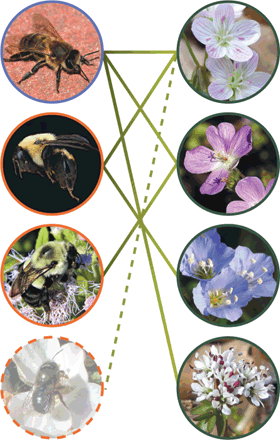
\includegraphics[scale=0.3]{Plant_polinisator.png}
\caption{Exemple d'un réseau plant-pollinisateurs} 
\end{figure}

\end{frame}
\section{Le modèle Poisson log-normal}
\begin{frame}
\frametitle{Le modèle Poisson log-normal}
$(\mu, \Sigma) \in \mathbb{R}^n \times \mathcal{M}_n(\mathbb{R})$\\
\vspace{0.5cm}
$(Y_1,...,Y_n) \sim \mathcal{PLN} (\mu,\Sigma)$  \\
\\
\begin{itemize}
\item  $Z \sim \mathcal{N}_n(0,\Sigma)$ une variable gaussienne  latente

\item$\forall i \in \{1,...,n\}, Y_i\mid Z_i \sim \mathcal{P}(\mathrm{exp}(\mu_i+Z_i))$\\

\item $(Y_i\mid Z )_{i \in \{1,...,n\}}$ sont indépendantes.
\end{itemize}
\end{frame}
\subsection{Avec les covariables et le offset}

\begin{frame}
\frametitle{Le modèle Poisson log-normal avec les covariables}
$X \in \mathbb{R}^d$ le vecteur de covariables.\\
$O \in \mathbb{R}^n$ le vecteur d'offset.\\
\vspace{0.5cm}
$(M, \Sigma) \in \mathcal{M}_{d \times n}(\mathbb{R}) \times \mathcal{M}_n(\mathbb{R})$\\
\vspace{0.5cm}
$(Y_1,...,Y_n) \sim \mathcal{PLN}_X (M,\Sigma)$  \\
\\
\begin{itemize}
\item  $Z \sim \mathcal{N}_n(0,\Sigma)$ une variable gaussienne  latente

\item$\forall i \in \{1,...,n\}, Y_i\mid Z_i \sim \mathcal{P}(\mathrm{exp}(O_i+X^T M^{(i)}+Z_i))$\\

\item $(Y_i\mid Z )_{i \in \{1,...,n\}}$ sont indépendantes.
\end{itemize}
\end{frame}
\subsection{Estimation des paramètres de la loi Poisson log-normale}
\begin{frame}
\frametitle{Estimation des paramètres de la loi Poisson log-normale :}
\begin{itemize}
\item \textbf{Maximum de vraisemblance :} densité de $\mathcal{PLN}(M,\Sigma)$ : $h_'(M,\Sigma)(Y_1,...,Y_n) = \int_{\mathbb{R}^n} \prod_{i=1}^n f_{(e^{O_i+X^T M^{(i)} + z_i})}(Y_i) g_{(0,\Sigma)}(z_1...z_n) \mathrm{d}z_1...\mathrm{d}z_n$.
\item \textbf{EM :} Pas de forme explicit de $p_{(\widehat{M},\widehat{\Sigma})}(Z_i \mid X_i)$ (\ref{Karlis2005})
\item \textbf{VEM :} Algorithme efficace mais pas de garantie assymptotique (\ref{Chiquet2017variational})
\end{itemize}
\end{frame}

\section{Composite likelihood}

\begin{frame}
\frametitle{Vraisemblance composite \ref{varin2008composite}}
\begin{center}
$\mathcal{CL}(Y)= \sum_{1\leq i <k \leq n} \mathrm{log} (h_{(M,\Sigma)}(Y_i,Y_k))$
\end{center}
 Fonction de densité en dimension 2 $ \longrightarrow $ intégrale sur $\mathbb{R}^2$.\\
\vspace{0.5cm}
Si on considère $N$ observations indépendantes et identiquement distribuées, on a :
\begin{center}
$\mathcal{CL}(Y)= \frac{1}{N}\sum_{j=1}^N \sum_{1\leq i <k \leq n} \mathrm{log} (h_{(M,\Sigma)}(Y^j_i,Y^j_k))$
\end{center}

$\rightarrow$ Estimateur par maximum de la vraisemblance composite. Consistance ? Normalité assymptotique ?
\end{frame}
\subsection{M-estimator}
\begin{frame}
\frametitle{Rappel sur les M-estimateurs : }
Un M-estimateur maximise une fonction de la forme 
\begin{center}
$\mathcal{M}_N : \theta \mapsto \frac{1}{N} \sum_{j=1}^N m_\theta(Y^j)$
\end{center}
Ici :  $m_\theta(Y^j) = \sum_{0 \leq i < k \leq n} \mathrm{log} ( h_{(M,\Sigma)}(Y_i^j,Y_k^j) )$
\end{frame}

\begin{frame}
\frametitle{Rappel sur les M-estimateurs : }
Un M-estimateur maximise une fonction de la forme 
\begin{center}
$\mathcal{M}_N : \theta \mapsto \frac{1}{N} \sum_{j=1}^N \sum_{0 \leq i < k \leq n} \mathrm{log} ( h_{(M,\Sigma)}(Y_i^j,Y_k^j) )$$
\end{center}
\paragraph{Consistance :}
\begin{theorem} \label{ThMest} \cite{vaart_1998}
Let $(\mathrm{M}_N)$ be a random sequence of functions in the variable $\theta$ and $M$ a determinist function in the variable $\theta$. If :
\begin{enumerate}
\item $\underset{\theta \in \Theta}{\mathrm{sup}} \mid \mathrm{M}_N(\theta)-\mathrm{M}(\theta) \mid \overset{\mathbb{P}}{\longrightarrow} 0$
\item the maximum $\theta^\ast$ of M is unique.
\end{enumerate}
Then any sequence of estimators $\widehat{\theta}_N$ with $\mathrm{M}_N(\widehat{\theta}_N) \geq \mathrm{M}_N(\theta^\ast)-\circ_p(1)$ converges in probability to $\theta^\ast$.
\end{theorem}

\paragraph{Normalité assymptotique}

\end{frame}

\begin{frame}
\frametitle{Consistance du maximum de la vraisemblance composite pour le modèle poisson log normal}
\begin{theorem}
The estimator $(\widehat{M}_N,\widehat{\Sigma}_N)$ constructed by maximizing the composite pairwise likelihood for $(Y^j_1,...Y^j_n)_{j \in \{1...N\}}$ is a consistent estimator of the correlation coefficients $M$ and of the matrix of variance-covariance $\Sigma$.
\end{theorem}
\begin{proof}
\begin{itemize}
\item
\end{itemize}
\end{proof}
\end{frame}


\end{document}